\section{Scaling Distributed Systems}

In practical applications, clusters of varying sizes are required. In some cases many nodes will be used, each replicating a small piece of data many times over. While in others, few nodes wil are used and larger chunks of data are replicated. Though in implementation, there are drawbacks to having a cluster with many nodes. As you continue to increase node number, various factors can lower a networks required time to reach consensus. Raft solves the consensus problem algorithmically, but let's, for example, take a look at a real world example where scaling comes into play.

We can imagine a large party of friends trying to decide where they want to go to eat for dinner. In this scenario in order to make an effective, and satisfying decision as to where the group should dine, each member of the group must be consulted. So the time in which it takes the entire group to come to an agreement increases as the size of the group increases.

In this large party, many more people will have to be consulted, and more options will have to be weighed before a choice is made. Though, compare this to just a few friends, who would be able to reach mutual agreement much faster, as they have less to consider, and fewer people that need to be taken into account before reaching a decision.

This principle is clearly demonstrated in distributed systems \cite{NeumanScaling}. Adding more nodes to a cluster makes it more difficult for the network to handle faults and replicate its state. Demonstrated in Raft, the more \textit{followers} in a system, the more heartbeats that have to be sent out to the \textit{leader}, processed, responded to, and then confirmed \cite{OngaroRaft}.


Though we can also demonstrate the benefits of a larger cluster. A greater number of nodes in a cluster allows for greater fault tolerance.
If we say there is a 25\% chance that a node fails at some point, we can model the probability of a cluster reaching agreement as such:


We define a function, $L(n)$, that is the probability a cluster of size $n$, can reach consensus given they have a 25\% of failing. Essentially equivalent to the common \textit{binomial cumulative density function}.

\[L(n) = 1- \sum_{i=0}^{n/2-1} {n \choose i}(0.75)^{i}(0.25)^{n-i}\]

With this function, we model the probability given each cluster size: 

\[\{(n, p): n \in \{3,5,7,...,51\}, p=L(n)\}\]

\vskip 0.25in

Producing a distribution as such:

\vskip 0.25in

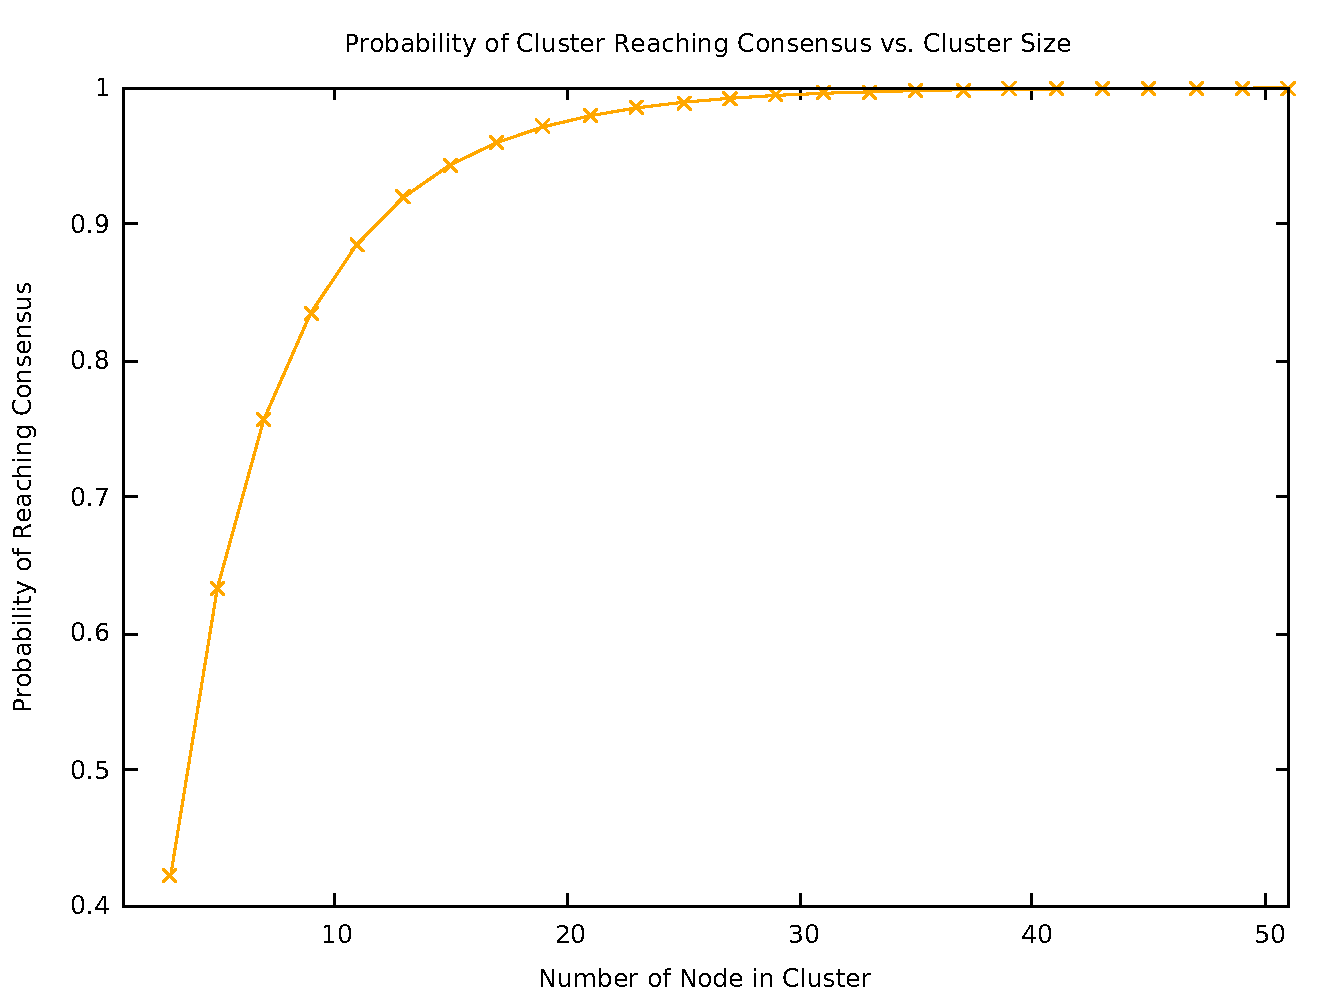
\includegraphics[width=0.5\textwidth]{cprob.pdf}


With this distribution we can see the theoretical benefits of a greater horizontal size. When increasing the number of servers, we initially see a great jump in the probability that the cluster reaches consensus. While this probability does increase, the servers quickly hit a point, in this instance at a size of about 30 servers, where the there are no observable benefits to fault tolerance.

Now we begin to look at some of the possible methods to scale distributed systems, each with varying degree of complexity and success.

\subsection{Non-Voting Servers}

One common way of increasing the capabilities of a large Raft cluster, is to change the voting status of additonal nodes.
Usually when we discuss creating larger clusters, we mean creating a cluster of servers, each with full voting priveleges.
But every one of these members all having full voting power, requires extra considerations in the cluster.
When you are a \textit{full} node, you must participate in log replication, as well as be consulted when changes need to be made to the replicated log.
So a common solution to this requirement for being a \textit{full} voting server, is making some of the members \textit{non-voting} servers.
This allows for the node to participate in the cluster, gaining the benefits of the log replication, but not bogging down the cluster by increasing the quorum size \cite{NonVoting}. 
Though it should be noted that this solution does not in any way solve the presented problem. Demoting nodes to a non-voting configuration, does not assist with the fault tolerance of the cluster. Supose you spin up a cluster with 5 full Raft servers, and 100 non-voting servers. If even just 3 of the full nodes fail, the system can no longer make progress, even though we have allocated resources for running a total of 105 servers because, the majority of the voting nodes have failed.

\subsection{Sharding}

There is also a way of scaling writes and reads. Some databases divide up the data their are trying to replicate using a process called \textit{sharding}. A great example of this process can be found in Google's Spanner database\cite{Spanner}. \textit{Sharding} works as a type of distributed load balances to balance the store of data across many consensus groups.

\subsection{Batching}

Other databases work to alter the process of sending or receiving inter-node messages. The Calvin database works to group messages, and specially schedule them in order to maintain consistency, and scalability \cite{Calvin}.